%!TEX root = volumeFinal.tex 
\chapter{\label{chap:busca}Busca}

Para encontrar uma sequência de ações que um agente baseado em objetivo consiga chegar ao seu objetivo é possível utilizar técnicas de Busca. O principio da busca é encontrar uma solução de um problemas através de um conjunto de ações que alcancem o objetivo desejado. Para utilizar as técnicas de busca é preciso formalizar o problema a ser resolvido e o objetivo a ser alcançado, pois na busca, como entrada é recebido um problema e é retornado uma solução na forma do conjunto de ações \cite{intelligence2003modern}. 

\section{Problema de busca}

Para entender melhor como funciona as técnicas de busca é preciso primeiro definir um problema. Um problema pode ser definido por cinco componentes \cite{intelligence2003modern}:
   
\begin{itemize}
	\item $S_{0}$ - O estado inicial, que o agente começa no ambiente;
	\item Ações- Conjunto das possíveis ações presentes no agente;
	\item Resultado(s, a) - Um modelo de transição, que define o estado resultando após a execução da ação a no estado s;
	\item Objetivo(s) - Verifica se o estado é o objetivo do agente;
	\item Custo do caminho - Uma função que defina um valor numérico para cada ação realizada em um estado. Essa função pode ser denotada por $c(s, a, s^{'})$, onde s é o estado atual do agente, a é a ação que será aplicada ao estado s e $s^{'}$ é o estado resultante aplicando o modelo de transição resultado(s, a). 
\end{itemize}   

Esses elementos definem um problema. Uma solução para um problema inicia no estado inicial, e através do modelo de transição utiliza ações para chegar ao objetivo do agente. Pelo fato de que as técnicas de busca aceitam mais de uma soluções para o mesmo objetivo, com conjuntos de ações diferentes, é utilizado para medir a qualidade da solução o custo do caminho, uma solução ótima é tida quando o menor custo do caminho de todas as soluções possíveis é encontrado utilizando o custo do caminho para cada ação realizada \cite{intelligence2003modern}.

Para exemplificar um problema de busca, considere o mapa apresentado na figura \ref{fig:mapabusca}, cada circulo representa uma cidade, para o exemplo considere o estado inicial como sendo a cidade de São Jerônimo, a ação disponível é se locomover entre as cidades que tenham ligação, o modelo de transição também são as ligações entre as cidades, o objetivo é chegar na cidade de Porto Alegre, e o custo de cada caminho está definido na transição. 

\begin{figure}[ht]
	\centering
	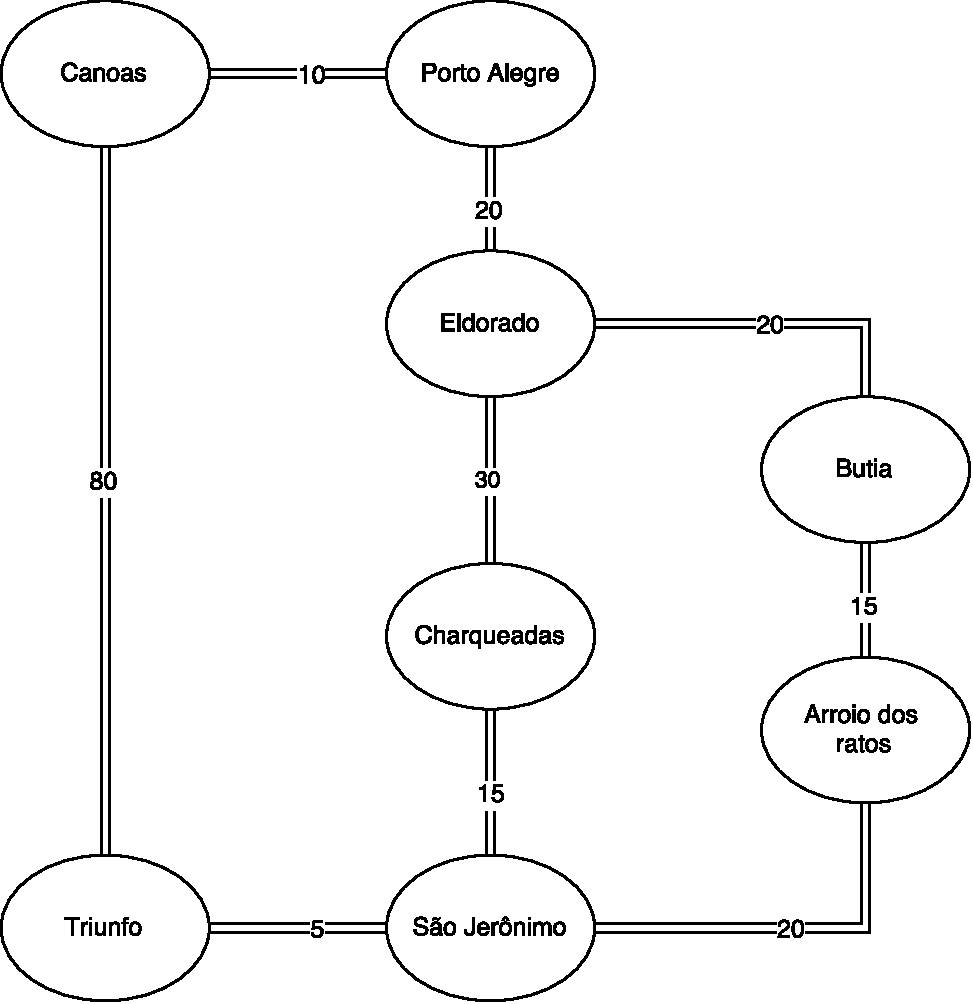
\includegraphics[width=0.6\textwidth]{fig/mapabusca.pdf}
	\caption{Mapa para o exemplo de problema de busca}
	\label{fig:mapabusca}
\end{figure} 

Para atingir o objetivo, utilizando uma busca, é preciso tentar os possíveis caminhos até o objetivo. Digamos que o agente comece sua viagem indo para a cidade de Triunfo, para nós, humanos, é intuitivo que a escolha não foi a melhor de inicio, mas a técnica só terá como saber após realizar todas as possíveis opções de caminhos, ou se utilizar de funções heurísticas, que acrescentam um conhecimento adicional para a resolução do problema \cite{intelligence2003modern}.

\section{Busca adversaria}

A busca adversaria é utilizada para ambientes competitivos, como nos jogos. Como em um jogo o jogador, preferencialmente, não informa suas jogadas previamente, o ambiente se torna imprevisível, e com isso os objetivos dos jogadores entram em conflito, ambos estão em busca da vitoria. Como solução para esse problema é preciso gerar uma solução de contingencia para tentar antecipar as jogadas do adversário. 	Jogos são difíceis de resolver com técnicas de IA, pois eles requerem uma habilidade de tomar alguma tipo de decisão, e as técnicas comuns as vezes não são satisfatórias, seja pelo fato dos estados que são possíveis de atingir ser muito grande, ou pelo curto espaço de tempo para tomar a decisão \cite{intelligence2003modern}. Para resolver esses problemas existem técnicas de busca adversaria para ambientes competitivos. Os problemas de jogos utilizam uma variação da definição de um problema de busca, totalizando seis componentes, são eles \cite{intelligence2003modern}:

\begin{itemize}
	\item $S_{0}$ - O estado inicial, que especifica como o jogo se configura no inicio.
	\item Jogadores(s) -  Define qual jogador tem o movimento no estado.
	\item Ações(s) - Conjunto das ações possíveis em um estado.
	\item Resultado(s, a) - Um modelo de transição, que define o resultado da ação a aplicada ao estado s.
	\item Terminal(s) - Verifica se o estado é um estado onde o jogo terminou.
	\item Utilidade(s,p) - Define qual é o valor numérico para o jogo quando atingir um estado s terminal por um jogador p. 
\end{itemize}

Com esses componentes descritos é possível entender alguma das técnicas de busca adversarias. 

\subsection{Minimax search}

Para explicar como é resolvido um problema pelo algoritmo de \textit{Minimax search}, primeiro é preciso considerar um jogo com dois jogadores, um é chamado de MAX e o outro de MIN. O jogador MAX representa o jogador que está tentando ganhar o jogo, e o jogador MIN é o jogador que está jogando contra. O jogo é alterna entre jogada de MIN e de MAX até o final do jogo, como em jogos por turnos. Quando são feitas jogadas que beneficiam o jogador MAX é obtido uma recompensa positiva e quando acontece ao contrario, o jogador MIN se beneficia da jogada, é obtido uma recompensa negativa \cite{intelligence2003modern}.
 
O estado inicial, as ações e os resultados definem a arvore das jogadas para o jogo. A arvore representa em cada nodo um estado do jogo e cada ligação com os níveis de baixo são os estados resultantes após a execução de cada ação possíveis para o estado. A alternância entre as jogadas de MAX e MIN até chegar as folhas da arvore, que correspondem aos estados terminais. Como o ponto de vista é do MAX, o valor de cada nodo folha representa o valor de utilidade para o MAX, e os maiores valores representam bons resultados para o MAX e ruins para o MIN. Com isso o caminho resultante indica que aquela ação será a melhor ação para o estado atual \cite{intelligence2003modern}. Um exemplo de uma arvore pode ser visto na Figura \ref{fig:gametree}, considerando os valores contidos nos nodos folhas o valor de utilidade do estado, a figura mostra que a técnica escolhe o melhor valor, neste caso o mais alto, para o jogador. 

%\msr[inline]{colocar uma figura de uma game tree?}
\begin{figure}[ht]
	\centering
	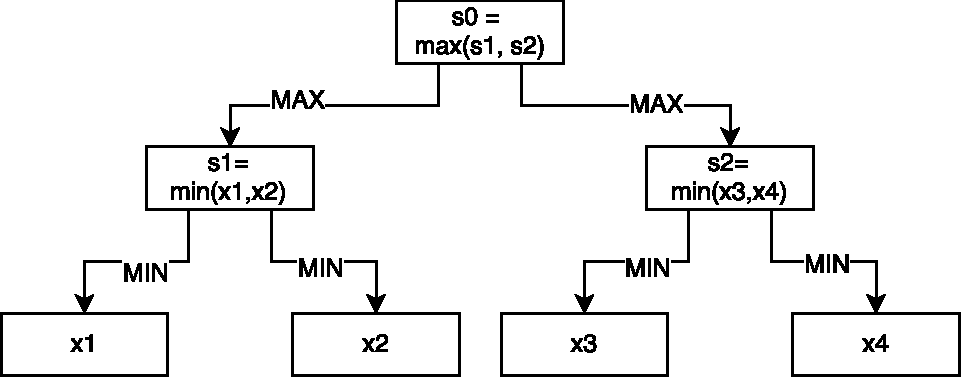
\includegraphics[width=0.6\textwidth]{fig/gametree.pdf}
	\caption{Exemplo de GameTree}
	\label{fig:gametree}
\end{figure} 

Este tipo de busca leva em consideração que o jogador adversário sempre realizará a jogada que mais lhe beneficiará. O algoritmo de \textit{minimax search} retorna a jogada que tem a melhor chance de resultar em uma vitoria no estado atual. O algoritmo sempre acha uma solução e ela é sempre a solução que, dentro das jogadas possíveis, é a melhor para o jogador \cite{intelligence2003modern}.  


%\subsection{Monte Carlo tree search}